\documentclass[a4paper,12pt]{report}
\usepackage{alltt, fancyvrb, url}
\usepackage{graphicx}
\usepackage[utf8]{inputenc}
\usepackage{float}
\usepackage{hyperref}
\usepackage{minted}
\usepackage{lineno}
\usepackage{array}
\usepackage{tabularray}
% Questo commentalo se vuoi scrivere in inglese.
\usepackage[italian]{babel}
\graphicspath{{./images/}}

\usepackage[italian]{cleveref}
\title{Relazione dell'elaborato di Basi di Dati
    \\ Sistema di gestione penitenziario}

\author{Leonardo Grimaldi}
\date{\today}   
\begin{document}
\maketitle
\tableofcontents
\chapter{Analisi}
\section{Introduzione}
Viene commissionata da un ente governativo la realizzazione di un software gestionale per una casa circondariale che faciliti il tracciamento di detenuti e loro spostamenti.
\section{Intervista}
\begin{linenumbers}
\modulolinenumbers[5]
Si chiede di realizzare un portale che consenta di gestire e storicizzare varie operazioni comuni di un carcere. Per i \textbf{detenuti} in arrivo si vogliono memorizzare gli estremi della persona.
%
I dati richiesti sono:
\begin{itemize}
    \item Nome, cognome, data di nascita, il numero della carta d'identità, altezza
\end{itemize}
Il carcere gestisce solamente detenuti italiani maggiorenni in possesso di carta d'identità quindi non occorre gestire il caso in cui essa non sia presente.
%
Un detenuto può essere rilasciato e rientrare nel carcere, ma anche decedere durante la sua permanenza.
%
Ai detenuti sono assegnate delle \textbf{celle} \underline{letto} in base alla disponibilità.
%
Esse hanno una capacità e più prigionieri possono risiedere al loro interno.
%
\par
Nel corso della loro permanenza le assegnazioni possono subire variazioni e si dovrà quindi tenere traccia degli \textbf{spostamenti}.
%
Questo include la data e ora di uscita e in quale cella è avvenuto lo spostamento.
%
All'interno della prigione sono presenti anche celle \underline{mediche} e \underline{solitarie} all'interno delle quali il prigioniero può risiedere temporaneamente.
%
Ogni cella appartiene a un \textbf{piano} che viene pattugliato da una o più \underline{guardie}.
%
Ogni piano fa parte di un solo \textbf{blocco}.
%
I \underline{turni di pattuglia} sono assegnati in base a un \textbf{orario} prestabilito in cui ogni giorno della settimana è formato da 3 turni:
\begin{itemize}
    \item Mattina: 06:00 - 14:00
    \item Pomeriggio/sera: 14:00 - 22:00
    \item Notte: 22:00 - 06:00 (del giorno successivo)
\end{itemize}   
La guardia lavorerà quindi per 8 ore al giorno con una pausa intermedia di 30 minuti e fine turno di 30 minuti.
%
Le pause e i cambi di turno non verranno gestiti dal database ai fini di copertura dell'orario, ma si suppone che vi sia una guardia di riserva che subentra temporaneamente.
%
\par Il \textbf{personale} del carcere è formato quindi da guardie, ma anche da \underline{amministratori} e di entrambi si vuole memorizzare: il nome, cognome, data di nascita, sesso e codice fiscale.
%
Gli amministratori sono le persone che hanno accesso al sistema gestionale e possono essere anche le guardie stesse.
%
Dovranno poter accedere al sistema con una password a loro assegnata.
%
Sia le guardie che gli amministratori possiedono un badge che li identifica univocamente all'interno della struttura.
%
Di loro si vuole memorizzare inoltre:
\begin{itemize}
    \item Nome, cognome, codice fiscale e sesso.
\end{itemize}
Il sistema non dovrà gestire la storicizzazione del personale e dei cambi di orario.
\end{linenumbers}
\section{Estrazione dei concetti principali}
Dall'intervista si possono estrapolare diverse figure che consentiranno di modellare lo schema concettuale.
\subsection*{Detenuto}
Sinonimi: prigioniero, carcerato
%
\\Persona rinchiusa nel carcere.
%
Ha una cella letto assegnata per tutta la permanenza.
%
\subsubsection*{Operazioni}
\begin{itemize}
    \item Trasferimento cella letto
    \item Spostamento temporaneo in celle mediche o solitarie
    \item Dichiarazione di decesso
\end{itemize}
\subsection*{Cella}
In generale, il luogo dove risiede il carcerato.
%
Ha una capacità massima e può essere di tre tipi: letto, medica e solitaria.
%
Può appartenere a un solo piano.
\subsection*{Piano}
Piano dell'edificio. In esso sono contenute molteplici celle.
%
Esso può essere controllato da una o più guardie.
\subsection*{Blocco}
Parte strutturale del carcere dove sono presenti un insieme di piani.
\subsection*{Personale}
L'insieme di persone che non sono detenuti, ma lavorano nel carcere e garantiscono la sicurezza e il suo corretto funzionamento.
%
Si dividono in guardie e amministratori e posseggono un badge.
\subsubsection*{Guardie}
Personale carcerario a cui è affidato il compito di controllare i piani in un certo turno del giorno 
\subsubsection*{Amministratori}
Personale che può accedere al sistema software gestionale attraverso una password.
%
Gli amministratori possono essere anche delle guardie.
\subsubsection*{Operazioni}
\begin{itemize}
    \item Inserimento guardie, assegnazione orario di lavoro
    \item Gestione detenuti: registrazione, trasferimento
\end{itemize}
\subsection*{Orario}
L'orario di lavoro che sarà assegnato alle guardie.
%
Avrà tre turni: mattina (06:00 - 14:00), pomeriggio (14:00 - 22:00) e notte (22:00 - 06:00).
\chapter{Progettazione concettuale}
\section{Schema scheletro}
%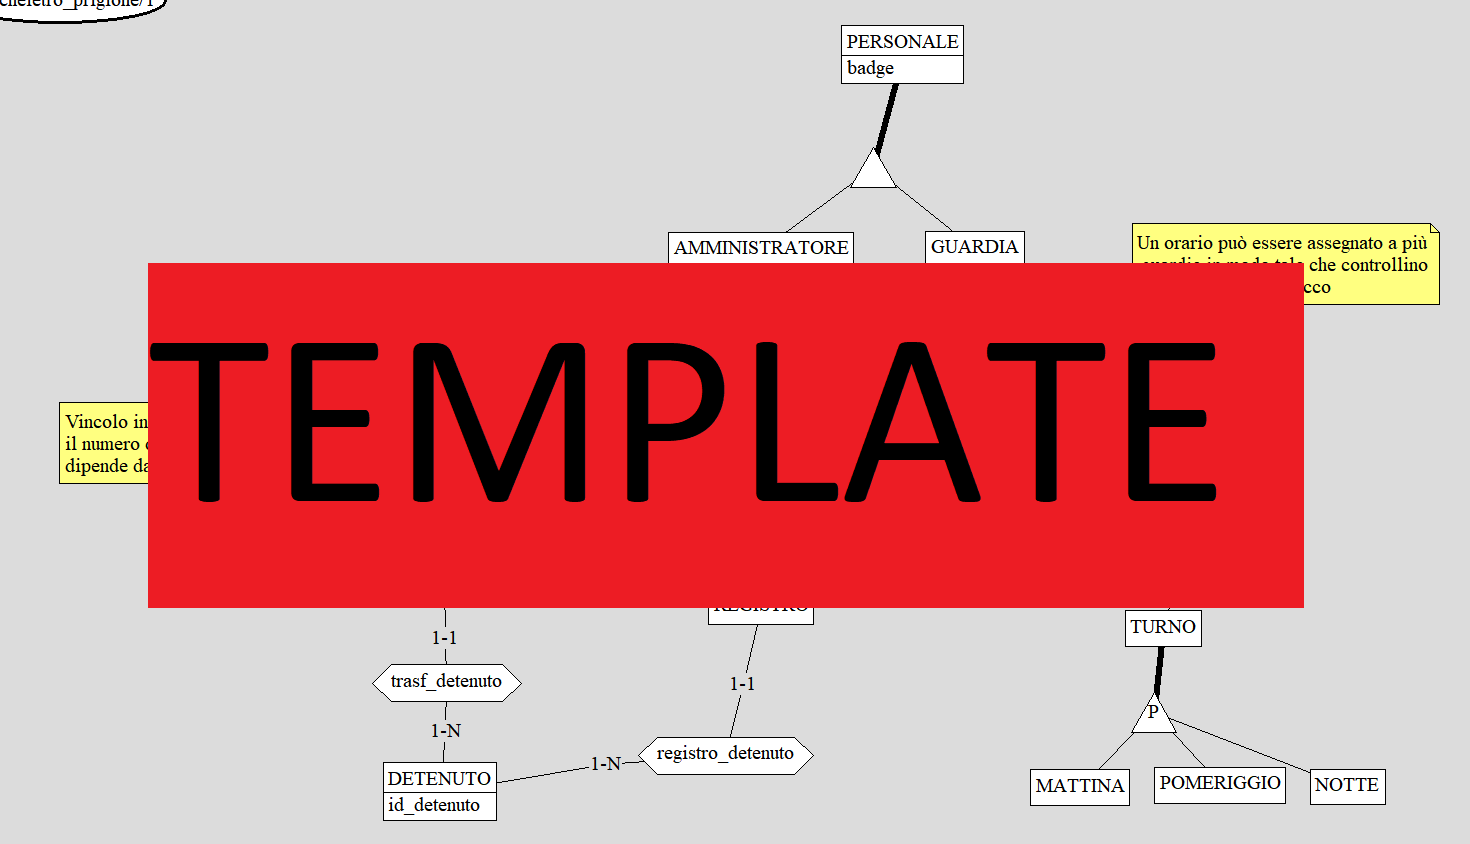
\includegraphics[angle=-90]{er_scheletro_prigione}
\section{Raffinamenti proposti}
Lo schema scheletro è una rappresentazione fedele ai concetti principali estratti nella sezione precedente, ma contiene anche un paio di elementi aggiuntivi che è stato necessario definire per modellare correttamente il dominio.
%
Innanzitutto si possono notare le tre nuove entità TRASFERIMENTO\_LETTO, RICOVERO e ISOLAMENTO che consentiranno di conservare le informazioni sui cambi di celle dei detenuti e ulteriori informazioni come la prognosi oppure il motivo.
%
Tutte queste hanno una cardinalità 1-1 sia dalla parte delle corrispondenti specializzazioni che da quella del REGISTRO\_DETENZIONE (introdotto nel seguente paragrafo) perché un TRASFERIMENTO non può esistere se manca un riferimento a chi e dove è stato spostato.
%
\par
Un'altra aggiunta importante è il concetto di REGISTRO\_DETENUTO; dall'intervista si è analizzato che un prigioniero potrebbe rientrare nel sistema e quindi si è creata la necessità di tenere traccia di questi.
%
Modellando così, un detenuto può essere reinserito nel sistema senza perdere informazioni sui suoi incarceramenti passati.
%
I TURNI, invece, sono in associazione 0-7 con l'ORARIO per esprimere il vincolo sul numero di giorni di una settimana (che infatti sono sette)
%
\par
L'entità REGISTRO\_ORARIO consente di storicizzare gli orari di lavoro delle GUARDIE per un certo PIANO.
%
Le cardinalità delle associazioni riferite a questa entità sono state ideate in modo tale da consentire a più GUARDIE di pattugliare un piano e una GUARDIA avere un solo PIANO da controllare in un ORARIO.
\section{Schema concettuale finale}
%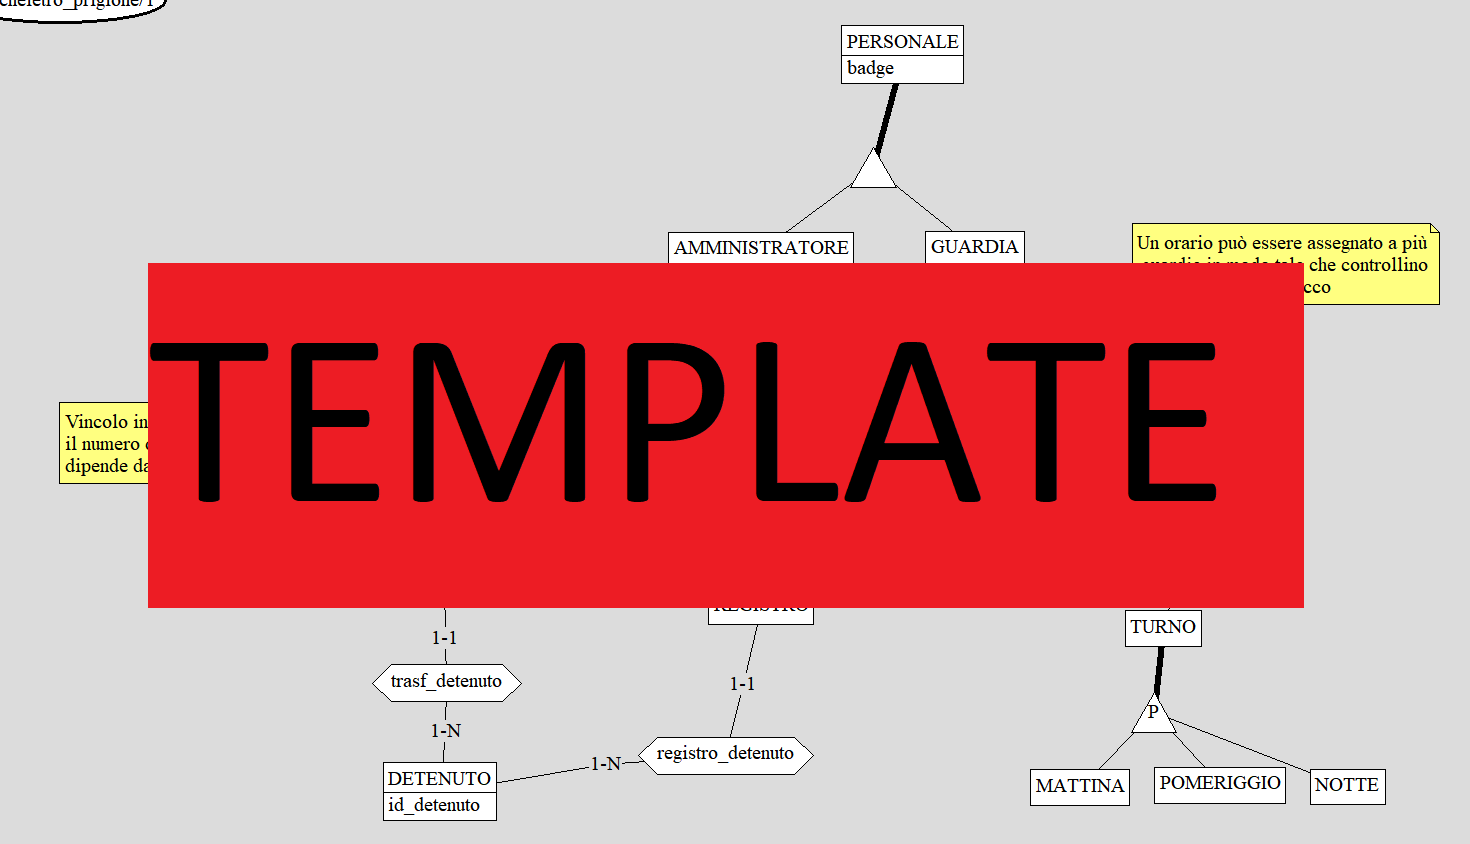
\includegraphics[angle=-90]{er_finale_prigione}
\chapter{Progettazione logica}ò
\section{Stima del volume dei dati}
Parlando con il committente.
%
La capacità del carcere è di 350 persone, di cui all'incirca 50 rientrano ogni tre anni.
%
Vi sono la sezione A e B con cinque piani e 35 celle ciascuna.
%
Inoltre, vi è anche la sezione C composta da due piani: il primo piano 10 celle mediche, il secondo 10 celle solitarie.
%


\begin{table}[H]
\begin{tabular}{lll}
\hline
Concetto & Costrutto & Volume \\ \hline
DETENUTO & E & 500 \\
assegnazione\_letto & A &  1000\\
TRASFERIMENTO\_LETTO & E &  1000 \\
trasf\_detenuto & A & 1000 \\
assegnazione\_letto & A & 1000\\
ISOLAMENTO & E & 200\\
spostamento\_solitaria & A & 200\\
isolamento\_detenuto & A & 200 \\
RICOVERO & E & 350 \\
spostamento\_medica & A & 350 \\
ricovero\_detenuto & A & 350 \\
registro\_detenuto & A & 700 \\
REGISTRO\_DETENZIONE & E & 700 \\
CELLA & E & 370 \\
MEDICA & E & 10\\
LETTO & E & 350 \\
SOLITARIA & E & 10 \\
cella\_piano & A & 370 \\
PIANO & E & 12 \\
piano\_blocco & A & \\
BLOCCO & E & 3 \\
controllo\_piano & A & \\
REGISTRO\_ORARI & E & \\
controllo\_guardia & A & \\
GUARDIA & E & 25 \\
AMMINISTRATORE & E & 10 \\
PERSONALE & E & 35 \\
orario\_controllo & A & \\
ORARIO & E & 21 \\
orario\_turno & A & 21 \\
TURNO & E & 3 \\
\end{tabular}
\end{table}
\section{Descrizione delle operazioni principali e stima della loro frequenza}
\begin{table}[H]
\begin{tabular}{p{9cm} p{2cm} p{1cm}}
\hline
Operazione & Frequenza & Tipo \\ \hline
Inserimento nuovo detenuto & 2/giorno &  \\
Cambio cella letto & 5/mese &  \\
Ricovero & 5/mese & \\
Isolamento & 3/mese & \\
Inserimento nel registro di un vecchio detenuto & 1/mese & \\
Inserimento nuova guardia & 5/anno & \\
Inserimento nuovo amministratore & 2/anno & \\
Cambio orario guardia & 6/mese & \\
Visualizzare la lista dei detenuti presenti & 50/giorno & \\
Visualizzare i detenuti rientrati in prigione & 2/mese & \\
Visualizzare l'andamento settimanale di nuovi detenuti & 60/giorno & \\
Visualizzare la lista di tutti i blocchi & 60/giorno & \\
Visualizzare i primi cinque detenuti che sono stati trasferiti in celle solitarie più volte & 2/mese &
\end{tabular}
\end{table}
\section{Schemi di navigazione e tabelle degli accessi}
\subsection{Inserire un nuovo detenuto}
\begin{table}[H]
\begin{tabular}{p{5cm} p{2cm} p{1cm} p{1cm}}
\hline
Concetto & Costrutto & Accessi & Tipo \\ \hline
DETENUTO & E & 1 & L \\
DETENUTO & E & 1 & S \\
REGISTRO\_DETENZIONE & E & 1 & S \\
registro\_detenuto & A & 1 & S \\

\end{tabular}
\end{table}
\end{document}